\begin{figure}[t]
    \vspace{-1mm}
    \centering
        \begin{minipage}{\linewidth}
            \begin{subfigure}{\linewidth}
                \centering
                \scalebox{0.82}{
                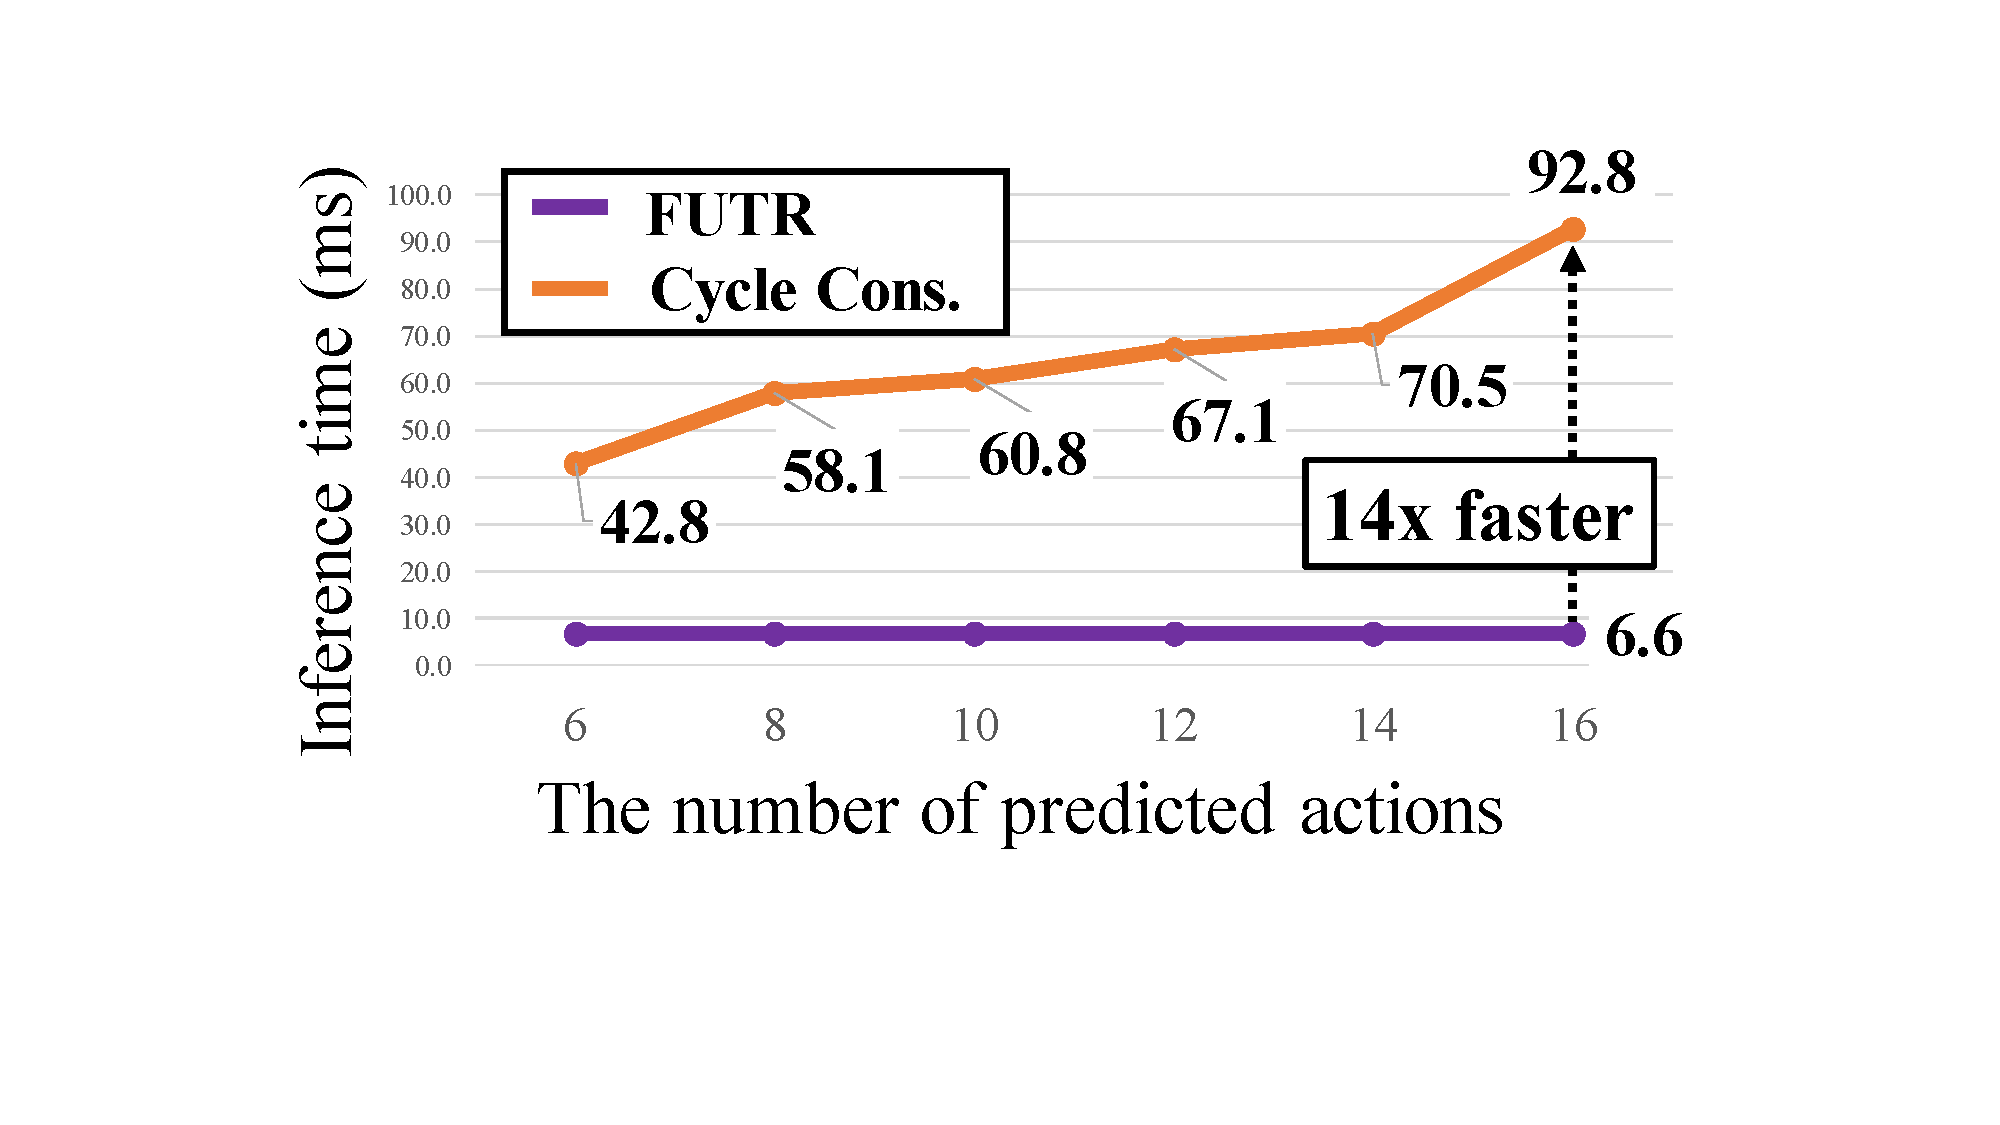
\includegraphics[width=\linewidth]{Figures/pdf/inf_cyc.pdf}
                }
                % \vspace{-5.5mm}
                \subcaption{\ours vs. Cycle Cons.~\cite{farha2020long}}
                \label{fig4:sub1}
            \end{subfigure}        
        \end{minipage}
        
        \vspace{2mm}
        
    \begin{minipage}{\linewidth}
            \begin{subfigure}{\linewidth}
                \centering
                \scalebox{0.8}{
                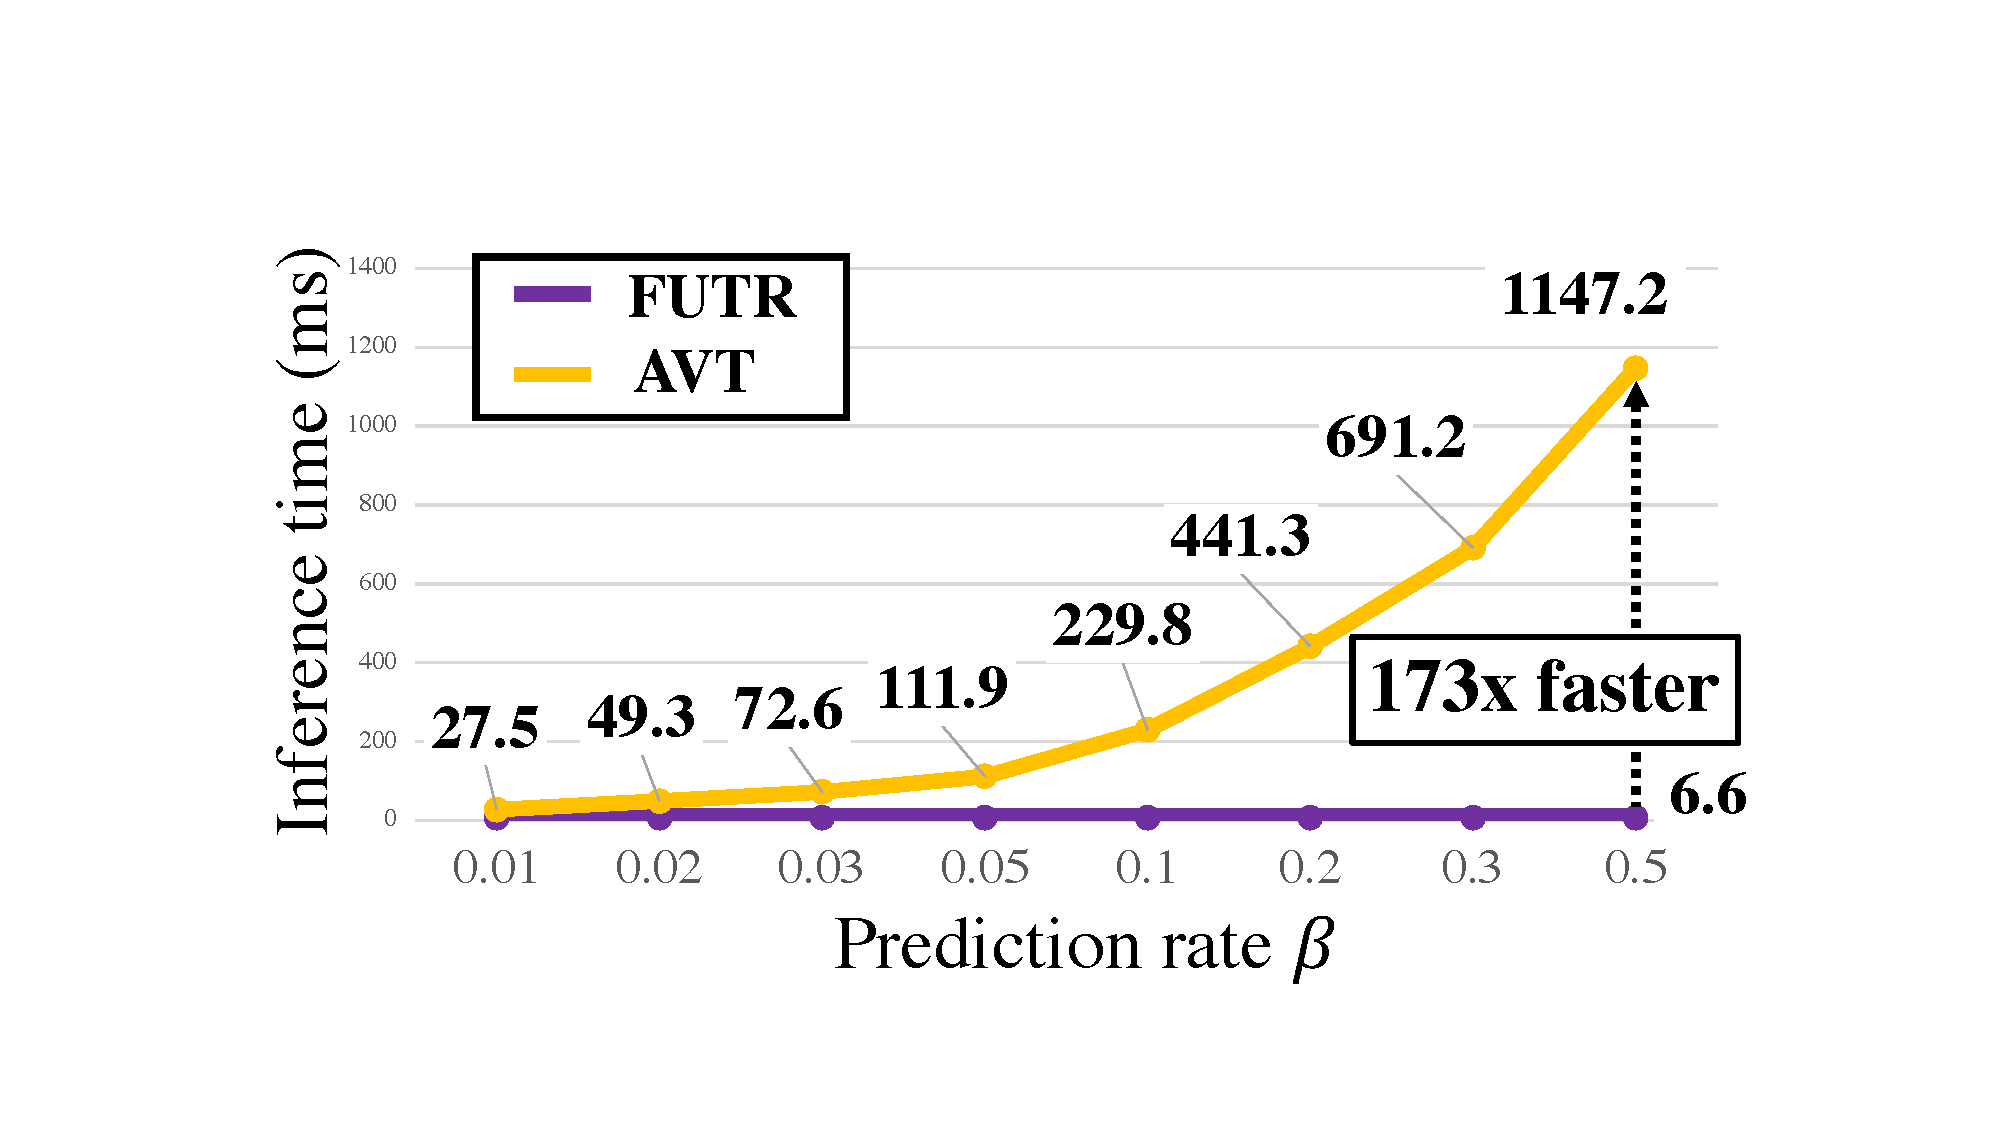
\includegraphics[width=\linewidth]{Figures/pdf/inf_avt.pdf}
                }
                % \vspace{-5.5mm}                
                \subcaption{\ours vs. AVT~\cite{girdhar2021anticipative}}
            \label{fig4:sub2}
            \end{subfigure}        
        \end{minipage}
    \vspace{-3.5mm}
    \counterwithin{figure}{section}
    \renewcommand\thefigure{S\arabic{figure}}
    \caption{\textbf{Inference time comparison with other methods}~\cite{farha2020long,girdhar2021anticipative}. Inference time of other methods linearly increases as the duration of the future action sequence to be predicted increases, \ie, the number of predicted actions or prediction rate $\beta$, increases, while that of FUTR is consistently fast.}
    \label{fig:inf}
    \vspace{-6mm}
\end{figure}